\documentclass[10pt,a4paper]{article}
\usepackage[utf8]{inputenc}
\usepackage[french]{babel}
\usepackage{amsmath,amsfonts,amssymb}
\usepackage{graphicx}
\usepackage{caption}
\usepackage{systeme}
\usepackage{subcaption}
\usepackage{esvect}
\usepackage{hyperref}
\usepackage[margin=0.5in]{geometry}
\usepackage{listings}
\usepackage{xcolor}

\definecolor{mGreen}{rgb}{0,0.6,0}
\definecolor{mGray}{rgb}{0.5,0.5,0.5}
\definecolor{mPurple}{rgb}{0.58,0,0.82}
\definecolor{backgroundColour}{rgb}{0.95,0.95,0.92}

\lstdefinestyle{CStyle}{
    backgroundcolor=\color{backgroundColour},   
    commentstyle=\color{mGreen},
    keywordstyle=\color{magenta},
    identifierstyle=\color{blue},
    numberstyle=\tiny\color{mGray},
    stringstyle=\color{mPurple},
    basicstyle=\footnotesize,
    breakatwhitespace=false,         
    breaklines=true,                 
    captionpos=b,                    
    keepspaces=true,                 
    numbers=left,                    
    numbersep=5pt,                  
    showspaces=false,                
    showstringspaces=false,
    showtabs=false,                  
    tabsize=2,
    language=C
}
\lstdefinestyle{customc}{
  belowcaptionskip=1\baselineskip,
  breaklines=true,
  frame=L,
  xleftmargin=\parindent,
  language=C,
  showstringspaces=false,
  basicstyle=\footnotesize\ttfamily,
  keywordstyle=\bfseries\color{green!40!black},
  commentstyle=\itshape\color{purple!40!black},
  identifierstyle=\color{blue},
  stringstyle=\color{orange},
}

\definecolor{comment}{RGB}{0,128,0} % dark green
\definecolor{string}{RGB}{255,0,0}  % red
\definecolor{keyword}{RGB}{0,0,255} % blue

\lstdefinestyle{c}{
	backgroundcolor=\color{backgroundColour},
	commentstyle=\color{comment},
	stringstyle=\color{string},
	keywordstyle=\color{keyword},
	basicstyle=\footnotesize\ttfamily,
	numbers=left,
	numberstyle=\tiny,
	numbersep=5pt,
	frame=lines,
	breaklines=true,
	prebreak=\raisebox{0ex}[0ex][0ex]{\ensuremath{\hookleftarrow}},
	showstringspaces=false,
	upquote=true,
	tabsize=2,
}


\begin{document}

\tableofcontents
\newpage
\section{Introduction}
Depuis plusieurs décennies, les microparticules et nanoparticules magnétiques, ainsi que leurs
suspensions ou gels, attirent l’attention des chercheurs et des industriels grâce à la possibilité
de changer leurs propriétés physiques et de les manipuler avec un champ magnétique externe.
En effet,  il existe une multitude de domaines dans lesquels leur utilisation s'avère être intéressante comme dans le milieu biomédicale. La maitrise de la suspension de ces micro et nanoparticules interviendrait dans la délibération/délivrance de manière contrôlé d'un médicament une fois ingéré, il serait également possible de séparer des cellules et des molécules biologiques associées à celles-ci. 
Ainsi dans certaines de ces applications, que cela soit dans le milieu biomédical ou dans un tout autre domaine, il y a une forte nécessité de séparer les micro ou  nanoparticules magnétiques du fluide suspendant en utilisant un filtre magnétique à haut gradient de champ magnétique.
\newline
\newline
C'est pourquoi le laboratoire FAST (Fluides, Automatique et Systèmes Thermiques), dont les sujets de recherches portent notamment sur  : l’hydrodynamique, la mécanique et la physique des milieux dispersés sur les fluides simples et multicomposants, les milieux dispersés macroscopiques (suspensions, granulaires, poreux) ainsi que sur la matière molle (polymères, colloïdes, gels…), a développé des outils de contrôle d’interfaces magnétiques basés sur le principe de la \textbf{lévitation magnétique}. L'objectif de ce projet est alors de développer un outil de calcul numérique permettant de prédire les effets de ces dispositifs.
\newline
\newline
Pour cela, il nous faut mettre en place une équation mettant en situation la lévitation magnétique que l'on cherche à étudier. Une fois que nous l'avons déterminé, nous allons résoudre par \textbf{méthodes numériques} cette équation afin de prédire la forme générale de l'interface.  
\section{Définitions}
Avant toute chose, il s'agit de définir plus précisément l'objet physique sur lequel nous allons travailler : \textbf{les ferrofluides}. Pour cela, il est tout d'abord nécessaire de parler de colloïdes.
\subsection{Colloïde}
Un colloïde est une dispersion d'une ou plusieurs substances suspendues dans un liquide, formant un système à deux phases séparées \cite{site1}. Il s'agit d'un mélange hétérogène de particules dont les dimensions vont du nanomètre au micromètre. On parle alors de \textbf{suspension} pour un colloïde et non de solution. 
\begin{center}
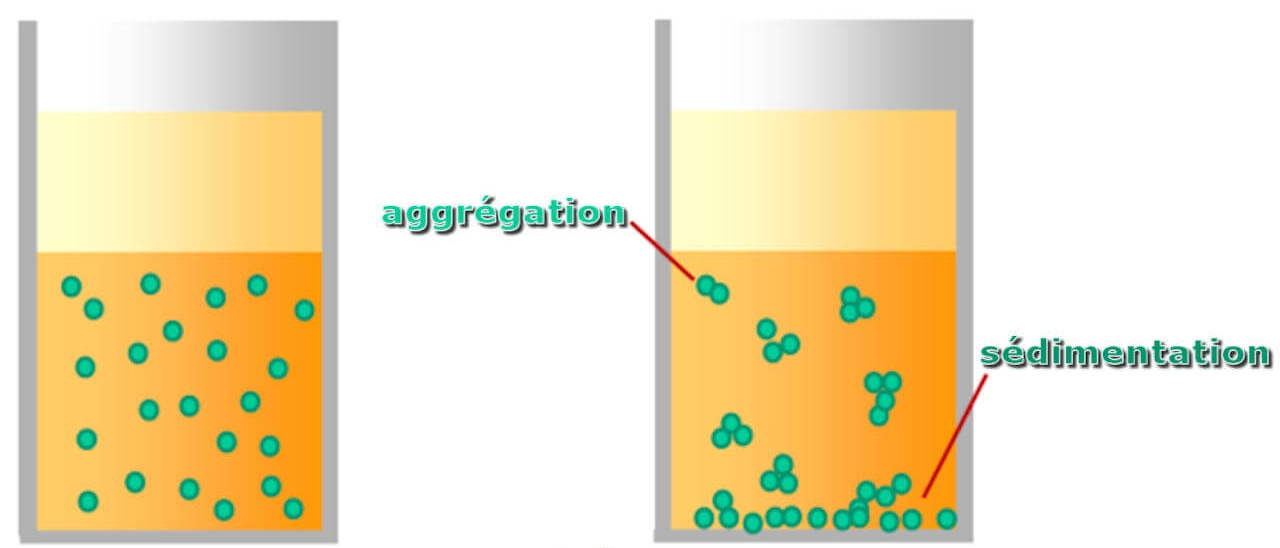
\includegraphics[scale=0.3]{images/solution-colloidale.jpg} 
\captionof{figure}{Suspension colloïdale \cite{site2}}
\end{center}
Par exemple les colles et les gels sont des colloïdes et forment des suspensions dites colloïdales. Les suspensions colloïdales sont intermédiaires entre les suspensions (particules de taille supérieure au micromètre) et les solutions vraies (particules de taille inférieure au nanomètre).
\newline
\newline
Parmi les colloïdes, on distingue deux grandes familles: les colloïdes stables et les colloïdes instables. La stabilité colloïdale est liée au changement de taille des particules (par exemple agrégation ou agglomération). Si les particules ne sont pas sujettes à des variations de taille, la dispersion est considérée comme colloïdale stable.
\begin{center}
\includegraphics[scale=0.25]{images/stabilité_colloidale.jpg}
\captionof{figure}{Stabilité colloïdale}
\end{center}
\subsection{Familles de composés magnétiques}
Afin de comprendre ce qu’est un ferrofluide, il est indispensable de préciser la définition des 3 grandes
familles de composés magnétiques: le diamagnétisme, le paramagnétisme et le ferromagnétisme \cite{olympiades}.
\newline
\newline
Tout d’abord, le \textbf{diamagnétisme} est une propriété générale de la matière atomique, qui provoque
l'apparition d'un champ magnétique opposé à un champ magnétique appliqué. Cet effet général, valable
pour toute matière (particulièrement visible sur le bismuth par exemple), est cependant d’intensité limitée et masqué par les éventuelles autres propriétés de paramagnétisme ou ferromagnétisme.
\newline
\newline
Le \textbf{paramagnétisme} désigne le comportement d'un milieu matériel qui ne possède pas d'aimantation
spontanée mais qui, sous l'effet d'un champ magnétique extérieur, acquiert une aimantation dirigée dans
le même sens que ce champ d'excitation. L’aimantation qui en résulte demeure cependant très faible car
l’effet de l’agitation thermique qui oriente aléatoirement les moments magnétiques reste prépondérant (exemple : ions fer III Fe3+, dioxygène O2)
\begin{center}
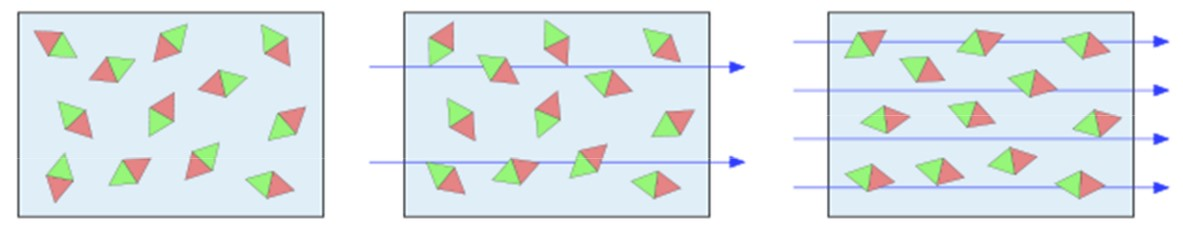
\includegraphics[scale=0.6]{images/diag_para_ferro_mag.jpg} 
\captionof{figure}{Sans excitation magnétique extérieur (1) Excitation magnétique peu intense (2) Excitation magnétique intense (3)}
\end{center}
Enfin, le \textbf{ferromagnétisme} est caractérisé par une aimantation spontanée (plus ou moins intense) et une réponse très intense à une excitation magnétique. Cependant, au-delà d’une certaine température propre à chaque matériau (appelée température de Curie), il existe une transition de ferromagnétique à paramagnétique.
\subsection{Ferrofluides}
Du point de vue microscopique, un ferrofluide est une suspension colloïdale stable de nanoparticules magnétiques dans un liquide porteur. Chaque particule porte un moment magnétique permanent. A l’échelle macroscopique, un ferrofluide est un fluide homogène que les particules magnétiques ont rendu noir. Lorsque l’on approche un aimant, le liquide est attiré dans son ensemble vers l’aimant. La réponse du ferrofluide à un champ magnétique est de type ferromagnétique.
\begin{figure}[!h]
    \centering
    \begin{subfigure}[b]{0.4\textwidth}
        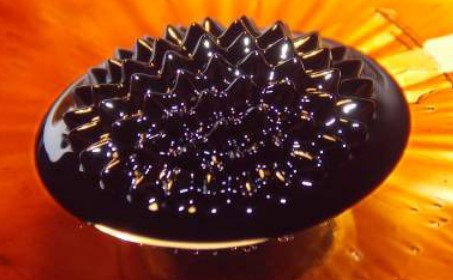
\includegraphics[width=\textwidth]{images/goutte_ferro.jpg}
    \end{subfigure}
    \begin{subfigure}[b]{0.4\textwidth}
        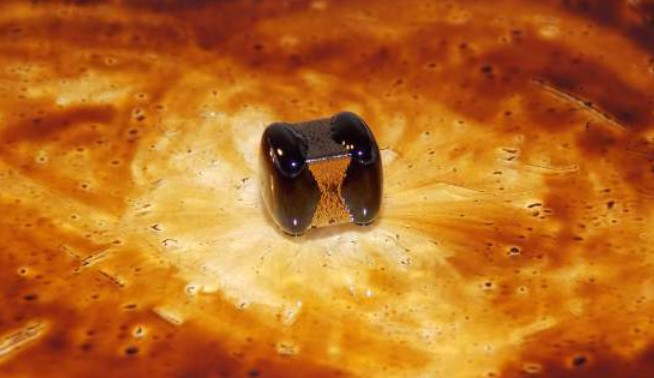
\includegraphics[width=\textwidth]{images/aimment_ferro.jpg}
    \end{subfigure}
    \begin{subfigure}[b]{0.4\textwidth}
        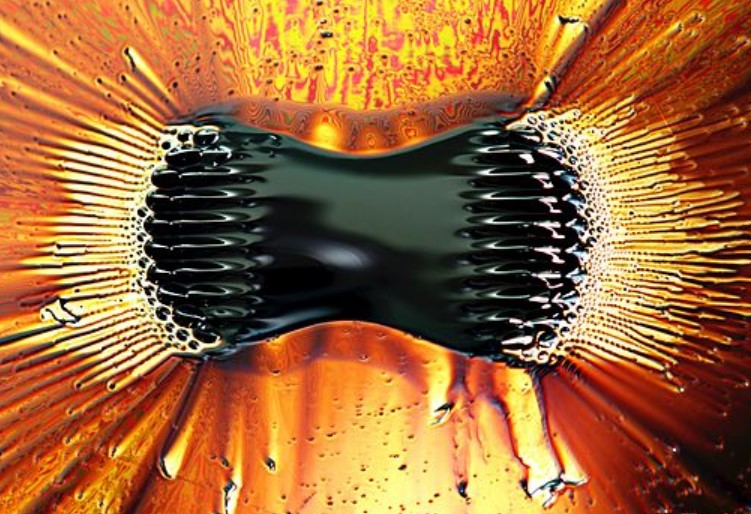
\includegraphics[width=\textwidth]{images/ferro.jpg}
    \end{subfigure}
    \caption{Ferrofluides soumis à un champ \cite{site3}}
\end{figure}

Dans la suite, il s'agit d'énoncer les différents phénomènes qui vont intervenir dans l'écriture de l'équation nécessaire pour prédire la forme de l'interface d'un ferrofluide soumis à un champ.
\section{Notions d'hydrodynamique}
\subsection{Tension de surface}
Les molécules à l'intérieur d’une phase condensée (liquide ou solide) sont soumises à des forces cohésives avec leurs voisines. Ces forces ne se font sentir qu’à de courtes distances, on les néglige donc la plupart du temps devant les autres forces. Néanmoins à petite échelle les forces de tension aux interfaces ne peuvent souvent plus être négligées devant les autres forces, ce qui est le cas dans notre projet.
\begin{center}
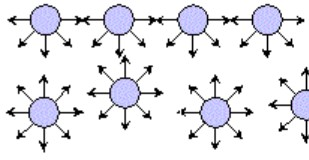
\includegraphics[scale=0.8]{images/tension.jpg} 
\captionof{figure}{Interactions entre les atomes au sein d'un liquide: tension de surface}
\end{center}
C'est ce phénomène de tension de surface qui explique par exemple que certains insectes puissent marcher sur l'eau.
\begin{center}
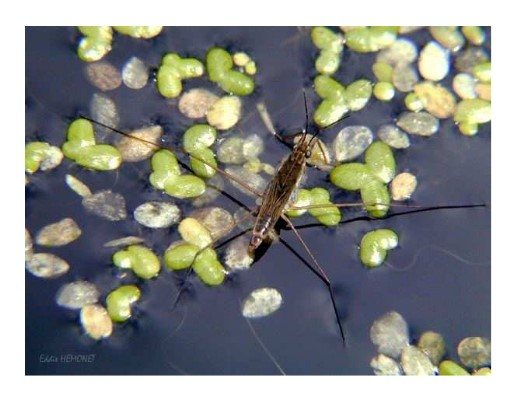
\includegraphics[scale=0.8]{images/insecte.jpg} 
\captionof{figure}{Gerris à la surface d'un étang}
\end{center}
Les phénomènes de tension de surface s'originent donc dans les forces intermoléculaires attractives qui existent dans toute phase condensée de la matière. Une molécule loin de la surface a donc plus de voisines donc une plus forte énergie d’interaction. A l'inverse, une molécule en surface a moitié moins de voisines de son espèce, donc moitié moins d’énergie d’interaction (voir figure ci dessus). L’énergie $E_S$ pour
fabriquer une surface S est égale à ce coût par molécule multiplié par le nombre de molécules en surface. \begin{equation}
E_s=\gamma *S
\end{equation}
Le coefficient $\gamma$ s'appelle la \textbf{tension de surface}.
\newline
\newline
C'est pourquoi chaque molécule dans les parties centrales du liquide a exactement la même force qui le tire de tous les côtés. Les molécules environnantes tirent la molécule centrale uniformément dans toutes les directions. Considérons maintenant une molécule de surface. Elle ne dispose plus que de forces agissant sur le liquide. Les forces adhésives air-liquide ne sont même pas aussi fortes que les forces de cohésion liquide-liquide. Ainsi, les molécules de surface sont attirées vers le centre du liquide, créant ainsi une couche compacte de molécules. Cette couche superficielle de molécules agit comme un film mince sur le liquide. C'est ce que l'on appelle la \textbf{tension de surface}.
\newline
\newline
Enfin, afin de minimiser son énergie surfacique, un fluide va avoir tendance à minimiser sa surface et donc à prendre une forme sphérique en l’absence d’autres contraintes.
\newline
\newline
Par la suite, comme l'on s'interresse à une allure d'interface, il est nécessaire d'étudier la courbure de celui-ci.
\subsection{Courbure}
La courbure d'un objet géométrique est une mesure quantitative du caractère « plus ou moins courbé » de cet objet. 
\newline
\newline
\underline{Par exemple :} dans le plan euclidien, une ligne droite est un objet à une dimension de courbure nulle et un cercle est un objet de courbure constante positive, valant 1/R (inverse du rayon). Dans l'espace euclidien usuel à trois dimensions, un plan est un objet à deux dimensions de courbure nulle, et une sphère est un objet à deux dimensions de courbure constante positive. Une « selle de cheval » possède au contraire une courbure négative.
\newline
\newline
Le rayon de courbure d'un tracé, en général noté R indique son niveau d'incurvation : plus le rayon de courbure est élevé, plus le tracé se rapproche d'une ligne droite, et inversement. Il est défini comme l'inverse de la courbure.
\newline
\newline
\begin{center}
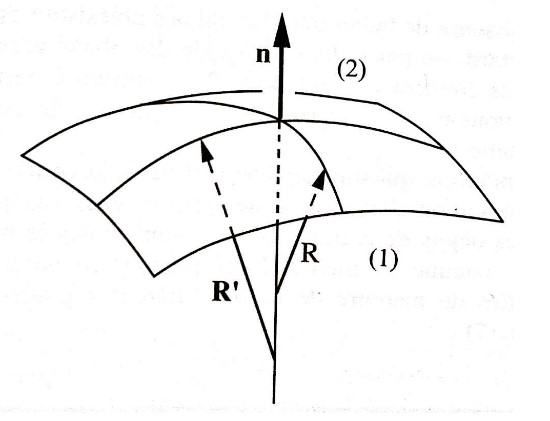
\includegraphics[scale=1]{images/courbure.jpg} 
\captionof{figure}{Courbure}
\label{fig07}
\end{center}
Si on considère le vecteur tangent à une surface (par exemple la figure \ref{fig07} ci-dessus) et qu'on déplace ce vecteur sur celle-ci, il va donc subir une rotation puisque la surface est courbée. Cette rotation est donc caractérisée par la courbure de la surface (y=f(x)) qui s'écrit:
\begin{equation}
C=\frac{y''}{(1+y'^2)^{\frac{3}{2}}}
\end{equation} 
\textbf{Remarque}: Une surface peut avoir des points de courbure nuls, c'est le cas d'un point selle.
\subsection{Angle de mouillage \cite{hydrodynamique}}
Dans de nombreuses situations, trois phases, solide-liquide-gaz par exemple, sont présentes et leur
frontière est une ligne nommée ligne triple. Si la ligne triple est stable, les trois forces interfaciales
doivent s'équilibrer. C'est notre cas, le ferrofluide est contenu dans un récipient il y a donc trois phases: air-récipient-ferrofluide. 
\newline
\newline
L'angle formé par la ligne triple et la phase solide est appelé angle de mouillage que l'on note $\theta$. Si cet angle est élevé, on est en \underline{situation non mouillante}, si cet angle est faible on est en \underline{situation mouillante}. Cett angle indique à quelle point le fluide s'étale sur le support.
\begin{center}
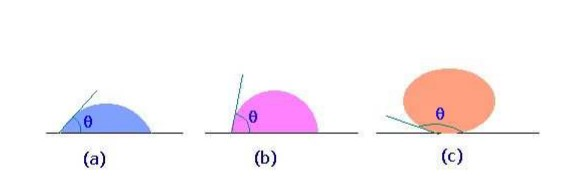
\includegraphics[scale=0.8]{images/mouillage.jpg} 
\captionof{figure}{Angle de mouillage}
\label{fig08}
\end{center}
C'est cet angle de mouillage qui donnera par la suite les conditions initiales pour résoudre l'équation décrivant l'interface du ferrofluide soumis à un champ magnétique. En effet, ce qui caractérise l'expérience faite, c'est le \textbf{ménisque formé entre le récipient et le ferrofluide} (pour chaque récipient ou ferrofluide différent on va obtenir un ménisque différent).
\begin{center}
\includegraphics[scale=0.8]{images/ménisque.jpg} 
\captionof{figure}{Ménisque}
\label{fig09}
\end{center}
\section{Notions d'électromagnétisme}
Par la suite, puisque l'on va soumettre le ferrofluide à un champ magnétique, il est nécessaire d'avoir quelques prérequis d'électromagnétisme pour mieux comprendre ce qu'il se passe et valider notre modèle. 
\subsection{Moment magnétique et Aimantation}
Le moment magnétique est une grandeur vectorielle qui permet de caractériser l'intensité d'une source magnétique. Cette source peut être un courant électrique, ou bien un objet aimanté. Par définition, le moment magnétique $\vv{\mu}$ d'un objet est défini comme le vecteur dont le produit vectoriel par l'induction magnétique externe B donne le moment de force $\vv{\tau}$ que subit l'objet. Cette relation se traduit mathématiquement par : 
\begin{equation}
\vv{\tau}=\vv{\mu} \wedge \vv{B}
\end{equation}
L'aimantation,  désignée par le symbole $\chi$ est définie comme la densité volumique de moment magnétique. Autrement dit:
\begin{equation}
\chi=\frac{d\mu}{dV}
\end{equation}
\subsection{Équations de Maxwell et théorème d'Ampère}
\begin{center}
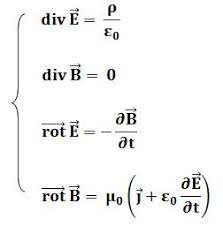
\includegraphics[scale=0.7]{images/equ_maxwell.jpg} 
\captionof{figure}{Equations de Maxwell}
\end{center}
Ensuite, à l'aide de ces équations, on obtient le théorème d'Ampere généralisé.
\begin{center}
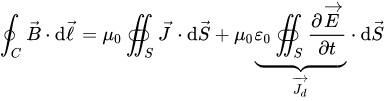
\includegraphics[scale=0.7]{images/theoreme_ampere.png} 
\captionof{figure}{Théorème d'Ampère généralisé}
\end{center}
\section{Équation de la surface}
\subsection{Configuration Étudiée}
On considère au départ un récipient rempli d'un \textbf{liquide ferromagnétique} Si on ne considère aucun champ au départ, alors le liquide est considéré comme étant à \textbf{l'équilibre hydrostatique}, seulement impacté par la gravité. Cependant si on soumet ce liquide à un champ magnétique, alors cette gravité est remplacée par une \textit{gravité effective} qui va alors dépendre de l'intensité du champ magnétique. Si celui-ci est variable spatialement et/ou temporellement, la gravité effective le sera aussi, et ainsi la hauteur du fluide va varier en fonction de la position et/ou du temps. 
\newline
\newline
Notre but est donc de prédire la forme du liquide obtenue en fonction du champ magnétique à l'aide de \textbf{résolutions numériques}. On l'étudiera dans un premier temps d'un point de vue théorique, puis on instaurera notre méthode de calcul de manière numérique.
\newline
\newline
Par ailleurs, on suppose dans un premier temps que l'allure de la surface est invariante selon y (voir schéma \ref{fig12} ci-dessous)
\begin{center}
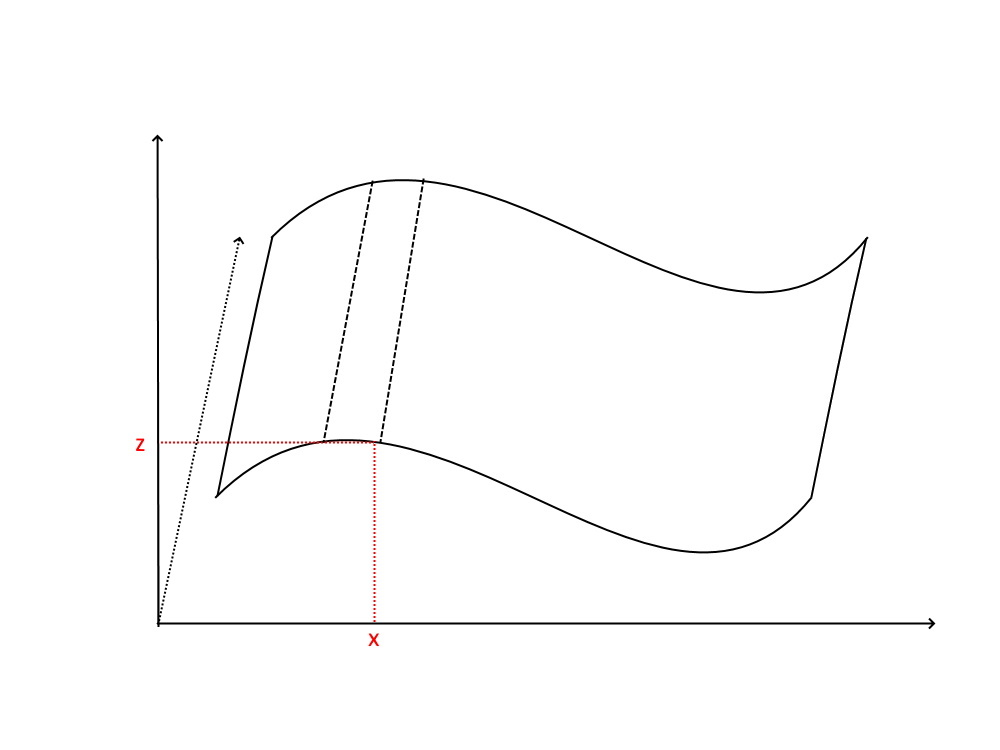
\includegraphics[scale=0.4]{images/IMG_4598.jpg} 
\captionof{figure}{Schéma de la situation}
\label{fig12}
\end{center}
On note $\eta (x)$ la hauteur de l'interface. Il s'agit par la suite de trouver cette hauteur.
\subsection{Équation associée}
Afin de prédire les formes que peut prendre l'interface, il nous faut déterminer une équation donnant la \textbf{hauteur en fonction du champ magnétique H et de la position dans le milieu}, autrement dit une équation du type \textit{$f(\eta$(x,H))=0}. 
\newline
\newline
Il nous faut tout d'abord prendre en compte les \textbf{ménisques} (figure \ref{fig09}) qui déterminent le système étudié (l'angle ne sera pas le même en fonction du ferrofluide et du récipient) et surtout car cela nous donne des conditions initiales sous forme de conditions limites qui garantissent l'unicité de la solution de l'équation que l'on va déterminer. 
\newline
\newline
Notre objectif ici est donc de déterminer cette équation.
\newline
\newline
La courbure $C(\eta)$ de la hauteur $\eta$ est tout d'abord décrite par (voir section 3.2):
\begin{equation}
C(\eta)=\frac{\eta\prime\prime}{(1+\eta\prime^2)^{\frac{3}{2}}}
\end{equation}
Cette courbure est alors influencée par deux facteurs: la pression de part et d'autre de l'interface et la tension de surface. En effet, en fonction de comment la pression varie, la surface du fluide n'aura pas la même allure et donc sa courbure aussi. De manière générale, on peut décomposer cette pression en deux parties: une partie constante dûe à la pesanteur ($P_g$) et une autre alternative dûe au champ magnétique auquel est soumis le fluide ($P_{mag}$).
\newline
\newline
De plus la tension de surface modifie également la courbure de l'interface. Sans elle, celle-ci se placerait de manière à avoir une pression égale de part et d'autre d'elle. La tension de surface agit alors comme un \underline{raidisseur}, d'où l'expression suivante avec la tension de surface $\gamma$:
\begin{equation}
\gamma*C(\eta)= P_{mag} - P_{g}
\end{equation}
Il convient enfin de déterminer l'expression de $P_{g}$ et $P_{mag}$.
Avec un principe fondamental de la statique des fluides on obtient l'expression de $P_{g}$ et avec des résultats classiques d'électromagnétisme, on obtient:
\begin{equation}
P_{g} = -\rho g\eta \indent
P_{mag}=E_{fmag}=-\chi*H(x,\eta)^2
\end{equation}
avec $\chi$ l'aimantation, $\rho$ la masse volumique, H le champ magnétique et g l'intensité de pesanteur.
(Le signe provient du paramétrage de l'espace choisi, ici z est vers le haut d'où le signe moins).
\newline
\newline
Enfin, il reste à prendre en compte le fait que l'on est à l'interface entre deux fluides (l'air et le ferrofluide). Il faut donc prendre en compte la masse volumique et l'aimantation des deux fluides, et en appliquant le principe fondamental de la statique à un morceau d'interface, on obtient l'équation suivante:
\begin{equation}
\frac{\gamma n\prime\prime}{(1+\eta\prime^2)^{\frac{3}{2}}} + (\rho_{1} - \rho_{2})g\eta + \frac{1}{2}(\chi_{1} - \chi_{2})H^{2}(x,\eta)=0
\end{equation}
Cette équation est donc une \textbf{équation différentielle non linéaire}. Pour simplifier dans un premier temps, nous nous sommes penchés sur deux cas particuliers : celui sans champ magnétique et celui pour une tension de surface nulle. De plus, on a les conditions limites aux parois de la cuve dûes aux menisques.
\section{Résolution numérique de l'équation}
\subsection{Résolution sans champ magnétique}
L'équation sans champ magnétique est la suivante:
\begin{equation}
\frac{\gamma \eta\prime\prime}{(1+\eta^{2}\prime)^{\frac{3}{2}}} + (\rho_{1} - \rho_{2})g\eta =0
\label{eq09}
\end{equation}
Avec les conditions limites citées précedemment.
\newline
\newline
Nous avons essayer d'avoir une intuition générale du comportement des solutions de l'équation en essayant de traiter des cas particuliers qui admettent une solution analytique. Nous avons donc décidé de regarder le cas particulier des solutions dans lesquelles $\eta\prime$ est très petit, de cette manière le terme $\frac{\gamma \eta\prime\prime}{(1+\eta^{2}\prime)^{\frac{3}{2}}}$ peut être approximé par $\eta\prime\prime$.
\newline
On se retrouve avec l'équation linéaire au $1^{er}$ ordre suivante:
\begin{equation}
\gamma \eta\prime\prime + (\rho_{1} - \rho_{2})g\eta =0
\label{eq10}
\end{equation}
\subsubsection{Résolution théorique de l'équation}
La résolution se fait en suivant les méthodes de résolution des équations différentielles linéaires du second degré.
\begin{equation}
\gamma r^{2} + (\rho_{1} - \rho_{2})g = 0
\end{equation}
Nous avons ainsi,
\begin{equation}
 \gamma r^{2}= (\rho_{2} - \rho_{1})g \iff  r^{2}=\frac{ (\rho_{2} - \rho_{1})g}{\gamma}
 \iff r = \pm \sqrt{\frac{ (\rho_{2} - \rho_{1})g}{\gamma}}
\end{equation}
On remarque que la grandeur $\sqrt{\frac{ (\rho_{2} - \rho_{1})g}{\gamma}}$ est l'inverse d'une longueur en analyse dimentionnelle. Pour faciliter les notations et avoir une interprétation physique des paramètres nous allons définir la longeur capilaire comme $l_{c} = \sqrt{\frac{\gamma }{(\rho_{2} - \rho_{1})g}}$
\newline\newline
Finalement  la solution est de la forme $\eta(x) = \alpha\exp({-\frac{ x}{l_{c}}}) + \beta\exp({\frac{ x}{l_{c}}})$
\newline
\newline
Il reste cependant à déterminer les constantes $\alpha$ et $\beta$. Pour cela on utilise les conditions limites $\eta\prime(0)$ et $\eta\prime(d)$.
Celles-ci désignent les pentes aux bords du récipient de longueur d et peuvent être déterminées grâce à l'angle de mouillage (voir Figure \ref{fig08}).
En effet comme on a supposé $\eta\prime \ll$ 1,  on peut en déduire que $\theta = \frac{\pi}{2} + \varepsilon$ avec $\theta$ l'angle de mouillage et où $\varepsilon \ll 1$.
\newline\newline
\begin{figure}[h]
	\centering
   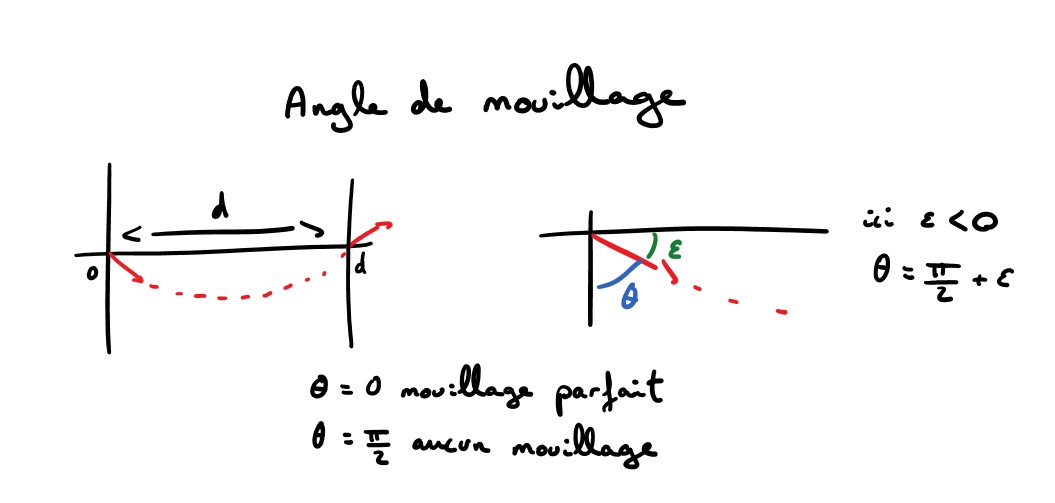
\includegraphics[width=11cm,height=6cm]{Schema1.JPG}
    \captionof{figure}{Schéma angle de mouillage}
    
\end{figure}
\newline\newline
On sait que $\eta\prime(0) = tan(\varepsilon)$  et $\eta\prime(d) = - tan(\varepsilon)$
\newline
De plus, 
\begin{equation}
	\eta\prime(x) =  -\frac{ 1}{l_{c}}\alpha\exp({-\frac{ x}{l_{c}}}) + \frac{ 1}{l_{c}}\beta\exp(\frac{ x}{l_{c}})
\end{equation}
\newline

D'où, $\eta\prime(0) = \frac{1 }{l_{c}}(\beta - \alpha)$
\newline

Et $\eta\prime(d) = \frac{ 1}{l_{c}}(\beta\exp({\frac{ d}{l_{c}}}) - \alpha\exp({-\frac{ d}{l_{c}}}))$
\newline

On résout donc le système suivant : 
\begin{equation}
(S) \Longleftrightarrow
\begin{cases}
\frac{1 }{l_{c}}(\beta - \alpha) &=tan(\varepsilon) \\
\frac{ 1}{l_{c}}(\beta\exp({\frac{ d}{l_{c}}}) - \alpha\exp({-\frac{ d}{l_{c}}})) &= -tan(\varepsilon)
\end{cases}
\end{equation}
\begin{equation}
\Longleftrightarrow
\begin{cases}
\beta - \alpha &=tan(\varepsilon)l_{c} \\
\beta\exp({\frac{ d}{l_{c}}}) - \alpha\exp({-\frac{ d}{l_{c}}}) &= -tan(\varepsilon)l_{c} \\
\end{cases}
\end{equation}
\begin{equation}
\Longleftrightarrow
\begin{cases}
\beta &=tan(\varepsilon)l_{c} + \alpha \\
(tan(\varepsilon)l_{c} + \alpha)\exp({\frac{ d}{l_{c}}}) - \alpha\exp({-\frac{ d}{l_{c}}}) &= -tan(\varepsilon)l_{c} 
\end{cases}
\end{equation}
\begin{equation}
\Longleftrightarrow
\begin{cases}
\beta &=tan(\varepsilon)l_{c} + \alpha \\
\alpha(\exp({\frac{ d}{l_{c}}}) - \exp({-\frac{ d}{l_{c}}})) &= -tan(\varepsilon)l_{c} (1 + \exp({\frac{ d}{l_{c}}}))
\end{cases}
\end{equation}
\begin{equation}
\Longleftrightarrow
\begin{cases}
\beta &=tan(\varepsilon)l_{c} + \alpha \\
\alpha &= \frac{ -tan(\varepsilon)l_{c} (1 + \exp({\frac{ d}{l_{c}}}))}{\exp({\frac{ d}{l_{c}}}) - \exp({-\frac{ d}{l_{c}}})}
\end{cases}
\end{equation}
\newline
On injecte $\alpha$ et $\beta$ dans l'équation et on obtient l'équation de la hauteur du liquide : 
\begin{equation}
	\eta(x)=-\exp({\frac{ -x}{l_{c}}})tan(\varepsilon)l_{c}\frac{ (1 + \exp({\frac{ d}{l_{c}}}))}{\exp({\frac{ d}{l_{c}}}) - \exp({-\frac{ d}{l_{c}}})} -\exp({\frac{ x}{l_{c}}})tan(\varepsilon)l_{c}\frac{1 + \exp({\frac{ -d}{l_{c}}})}{\exp({\frac{ d}{l_{c}}}) - \exp({\frac{ -d}{l_{c}}})}
\end{equation}


\subsubsection{Résolution numérique de l'équation}

Pour résoudre numériquement l'équation linéarisée du problème, nous avons appliqué la méthode d'Euler explicite \cite{euler} à notre équation de manière à voir que l'on retrouve bien la solution analytique que l'on connait. Il s'agira par la suite d'appliquer cette méthode à la vraie équation. 
\newline\newline
On part de l'équation \ref{eq10} et on pose :
\begin{equation}
u(x)=\begin{pmatrix}
   \eta(x)  \\
   \eta\prime(x)
\end{pmatrix}
u\prime(x) = f(x,u(x)) = \begin{pmatrix}
   \eta\prime(x)  \\
   -\frac{(\rho_{1} - \rho_{2})g}{\gamma}\eta(x)
\end{pmatrix}
\end{equation}
D'où la méthode d'Euler explicite :
\begin{equation}
\begin{cases}
u_{0} &=\begin{pmatrix}
   \eta(0)  \\
   \eta\prime(0)
\end{pmatrix} \\
u_{n+1} &= u_{n} + hf(x_{n},u_{n})\\
\end{cases}
\Longleftrightarrow
\begin{cases}
u_{0} &=\begin{pmatrix}
   \eta(0)  \\
   \eta\prime(0)
\end{pmatrix} \\
\begin{pmatrix}
   \eta_{n+1}  \\
   \eta\prime_{n+1}
\end{pmatrix}  &= \begin{pmatrix}
   \eta_{n} +h \eta^{\prime}_{n}  \\
   \eta\prime_{n} - h \frac{(\rho_{1} - \rho_{2})g}{\gamma}\eta_{n}
\end{pmatrix}
\end{cases}
\end{equation}

Nous avons par la suite considéré une interface huile/eau et utilisé les valeurs suivantes pour pouvoir implémenter en python nos différents résultats : 
\newline
\begin{itemize}
	\item $\rho_{2} = 920 kg.m^{3}$ pour l'huile d'olive
	\item $\rho_{1} = 1000 kg.m^{3}$ pour l'eau
	\item $\gamma = 0.018 N.m^{-1}$ pour la tension de surface entre l'eau et l'huile
	\item  $l_{c} = \sqrt{\frac{\gamma }{(\rho_{2} - \rho_{1})g}}$
	\item $d = 10l_{c}$
	\item $\epsilon = -0.1$
\end{itemize}
\vspace{1cm}
Cependant, il faut veiller à prendre des valeurs qui rentre de notre domaine d'utilisation. En effet, si la longueur d de la cuve est trop grande par rapport à $l_{c}$ les erreurs d'arrondi vont faire que nous perdrons de l'information d'un menisque vers l'autre. Pour notre code, c'est à partir de $d >35l_{c}$ que la précision machine n'est plus capable de suivre.
\newline
\newline
Nous avons donc un schéma récursif qui permet de calculer une approximation de tous les points de l'interface à condition de connaitre le point initial $\eta(0)$. Or, dans notre cas, nous ne connaissons pas ce point puisque nos conditions limites portent sur $\eta\prime$ aux bords de la paroi. 
\newline
C'est pour cela que, dans un premier temps, nous allons verifier la qualité de notre approximation et de notre calcul numérique en utilisant le résultat analytique pour nous donner l'information qui nous manque, i.e $\eta(0)$. Et nous retrouvons bien la fonction de la hauteur du liquide (Figure \ref{fig14_1})
\newline
On remarque cependant qu'en prenant une valeur différente, par exemple 0.0004, qui a une erreur de $20 \%$ par rapport à la valeur analytique, on se retrouve alors avec une erreur de $200000 \%$ à l'autre paroi de la cuve. Ceci prouve que ce système à une forme d'instabilité liée à l'instabilité intrinsèque de la méthode d'Euler elle même, en effet chaque pas cumule les erreurs de tous les pas précédents. 
\newline\newline
Ainsi, nous avons cherché à faire une étude de convergence afin que la méthode choisie ne soit plus dépendante du pas. Nous avons donc comparé le $\eta'(d)$ trouvé avec Euler avec la condition limite $\eta'(d)$, en cherchant une erreur inférieure à $5 \%$. Le pas de convergence trouvé : h= 4.48*10$^{-5}$ se trouve dans cet intervalle de convergence. 
\newline\newline
\begin{minipage}[c]{.46\linewidth}
     \begin{center}
             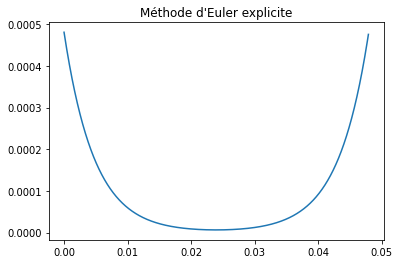
\includegraphics[width=7cm]{Euler_eta0.png}
             \captionof{figure}{Euler avec valeur analytique}
	     \label{fig14_1}
         \end{center}
   \end{minipage} \hfill
   \begin{minipage}[c]{.46\linewidth}
    \begin{center}
            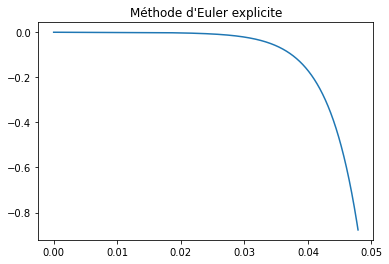
\includegraphics[width=7cm]{Euler_1.png}
            \captionof{figure}{Euler $\eta(0)$=0.0004}
        \end{center}
 \end{minipage}
\vspace{1cm}

Cependant, l'utilisation de la méthode d'Euler est faite en supposant que nous ne connaissions pas $\eta(0)$.
\newline
C'est pourquoi nous avons ensuite implémenté une méthode de dichotomie sur notre schéma d'Euler pour retrouver la valeur $\eta(0)$. De la même manière que l'étude de convergence nous avons comparé le $\eta'(d)$ trouvé à la condition limite $\eta'(d)$, puis resserré l'intervalle pour finalement atteindre $\eta(0)$ avec une précision de 10$^{-4}$.

\begin{figure}[h]
	\centering
    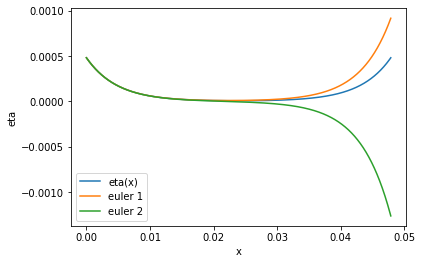
\includegraphics[width=.5\linewidth]{errreur.png}
    \captionof{figure}{Méthode de dichotomie}
    
\end{figure}

\newpage
Finalement, nous avons calculé l'erreur de notre méthode par rapport à la solution exacte trouvée précédemment. Nous avons ainsi, pour différents pas, calculé la moyenne de l'erreur en chaque point du schéma d'Euler et tracé celle-ci en loglog. Nous avons également tracé le seuil d'erreur à $10 \%$ afin de déterminer le pas optimal correspondant à celui-ci, qui est de 0.00021.

\begin{figure}[h]
	\centering
    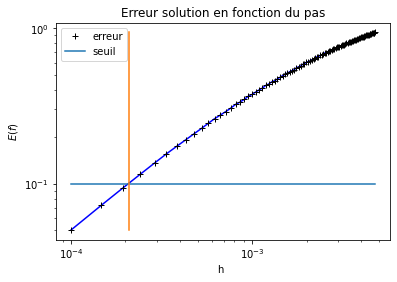
\includegraphics[width=.5\linewidth]{graph_Erreur.png}
    \captionof{figure}{Courbe de l'erreur en loglog}
    
\end{figure}

Notre courbe montre bien que plus le pas h diminue, plus l'erreur diminue également. Donc la solution trouvée à partir de la méthode d'Euler explicite converge vers la solution exacte. On peut alors conclure que cette méthode est plutôt efficace pour retrouver la fonction de la hauteur du fluide. Toutefois, il faudrait diminuer la precision des données afin que celles-ci n'engendrent pas une accumulation d'erreur et nous pourrions également envisager l'utilisation d'une autre méthode comme celle de \textbf{Runge-Kutta} pour une meilleure efficacité. Enfin, il faudrait tenter d'appliquer la même méthode que celle vue précédemment, non plus sur des cas particuliers, mais sur l'équation sans champs magnétique vue au début de cette partie (équation \ref{eq09}). 
\newline
\subsection{Résolution sans terme différentiel}
L'équation sans terme différentiel est donc la suivante:
\begin{equation}
(\rho_{1} - \rho_{2})g\eta + \frac{1}{2}(\chi_{1} - \chi_{2})H^{2}(x,\eta)=0
\end{equation}
Cette équation est une équation algébrique où il convient de trouver $\eta$ pour un champ donné. Il nous a donc fallu déterminer des expressions de champs magnétiques puis élaborer une stratégie de résolution numérique. Cette fois-ci, les conditions limites sont \textbf{sur H}. Il est donc nécessaire d'expliciter les différents champs magnétiques que nous avons utilisé afin d'en déterminer les conditions limites.

\subsubsection{Champs magnétiques: Nappe de courant}
La nappe de courant est le champ le plus simple à mettre en place, car si on envoie le courant selon Oy, alors on n'a plus qu'un \textbf{champ le long de Oz}. L'équation établie et implémentée est la suivante \cite{site4}: 
\begin{equation}
H(M) = \frac{jS}{2}\vec{u_{z}}
\label{eq08}
\end{equation}
\begin{figure}[h]
	\centering
    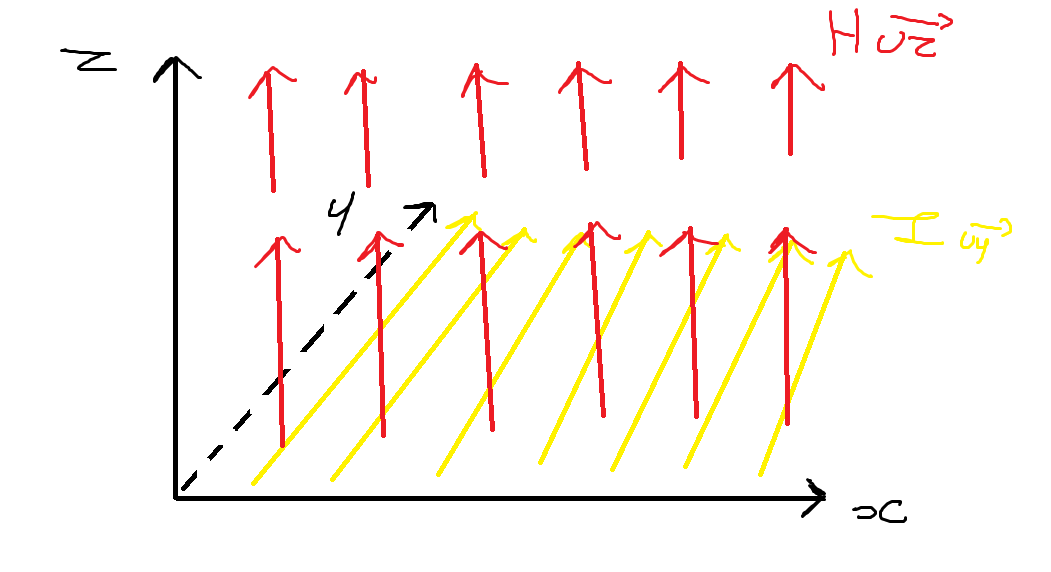
\includegraphics[width=.5\linewidth]{img_yamato/Nappe.png}
    \captionof{figure}{Nappe de courant}
    
\end{figure}
Avec j le \textit{courant surfacique} et S la \textit{surface de l'objet}. \\
Ici, nous avons un champ constant, qui ne dépend pas de la position du point M considéré, et surtout \textbf{qui ne tend jamais vers $+\infty$}. On n'a donc aucune condition limite sur ce champ.
\newpage
\subsubsection{Champs magnétiques : Fils }
Nous nous placons dans la situation où nous avons deux fils parallèles parcourus par un même courant dans des sens opposés.
\begin{figure}[h]
	\centering
    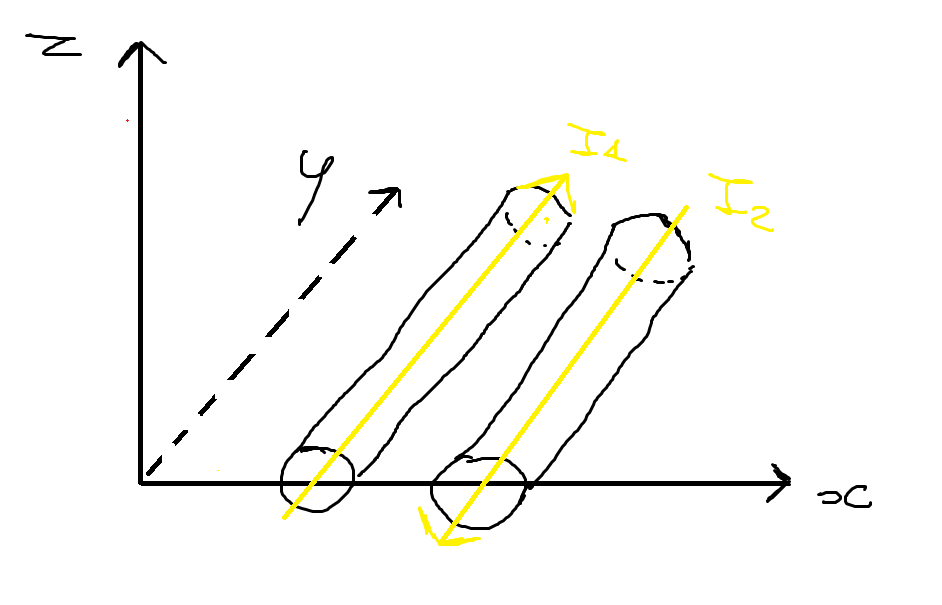
\includegraphics[width=.4\linewidth]{img_yamato/Fils.png}
    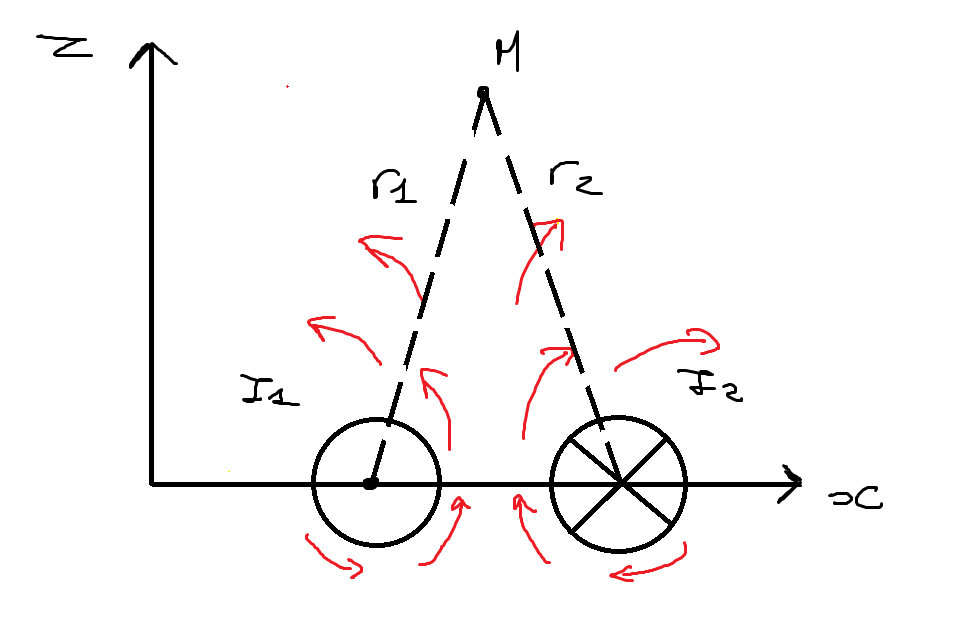
\includegraphics[width=.4\linewidth]{img_yamato/Fils2.png}
    \captionof{figure}{Fils à courant inverse}
\end{figure}
\newline
Le champ généré par deux fils de courant est plus complexe à établir car leur champ est la plupart du temps en coordonnées cylindriques (la géométrie de la situation y est plus adaptée), et nous avons voulu l'exprimer en coordonnées cartésiennes pour recoller par la suite à notre schéma numérique. Encore une fois, nous avons fait en sorte d'avoir une \textbf{invariance selon y}. Cela nous donne les formules suivantes \cite{site5} :

\begin{equation}
r = \sqrt{(x-x_{M})^2 + (z-z_{M})^2} \indent\indent H = \frac{I}{2\pi r}
\label{eq24}
\end{equation}
En considérant r la \textit{distance entre le point M et le fil considéré}. Etant donné que nous connaissons la position de nos deux fils, on peut facilement retrouver cette distance à l'aide d'un \textbf{théorème de Pythagore}.
\newline
On applique ces deux calculs pour obtenir les deux champs magnétiques crées par les fils 1 et 2. Pour obtenir le champ magnétique total de ces deux fils de courant, il suffit d'additionner les deux champs créés :
\begin{equation}
H = H_{1} + H_{2}
\label{eq25}
\end{equation}

On remarque facilement que si r \textrightarrow 0, alors \textbf{H \textrightarrow $+\infty$}. Pour remédier à cela, lorsque $r << 1$ (donc lorsque H prend une valeur trop importante), alors nous remplaçons la formule du fils de courant par la \textbf{formule d'une spire de courant} (car nous considérons que nous sommes là \textbf{à l'intérieur} du fil).
\newline
Dans ce cas là, la formule du champ est donc la suivante :
\begin{equation}
H = \frac{I}{2\pi R}
\label{eq11}
\end{equation}
avec R le \textit{rayon du fil}, qui est lui bien constant.
\newpage
\subsubsection{Champs magnétiques: Dipôle magnétique}
Il s'agit là d'un \underline{cas particulier des deux fils à courant inverse}. En effet, plus la situation est observée de loin, plus la distance entre les deux fils est petite \textbf{par rapport à la distance d'observation}. En pratique, cela revient à considérer que nos \textbf{deux fils sont superposés}. Cela nous donne le schéma suivant :
\begin{figure}[h]
	\centering
    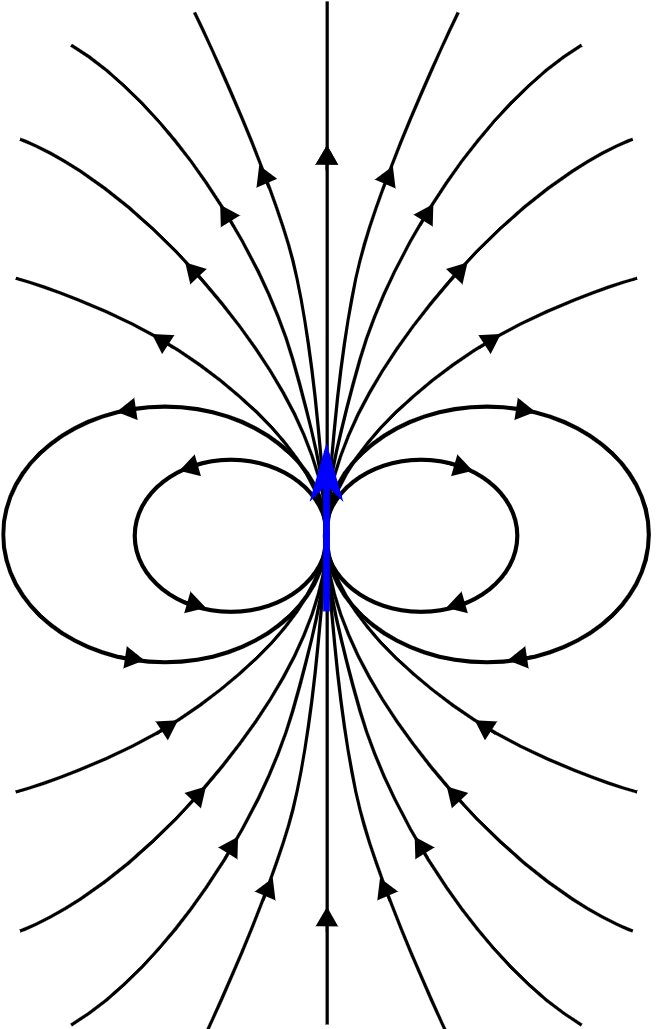
\includegraphics[width=.3\linewidth]{img_yamato/Dipole.png}
    \captionof{figure}{Dipôle magnétique}
\end{figure}
\newline
Le champ magnétique du dipôle magnétique en coordonnées cartésiennes sont donnés à partir du \textbf{moment dipolaire m} tel que  $m=I*S$, avec I \textit{l'intensité} et S la \textit{surface des bases du fil} \cite{site6}:
\begin{equation}
H_{x} = \frac{m}{4\pi}\frac{3zx}{r^5}\indent\indent H_{y} = \frac{m}{4\pi}\frac{3zy}{r^5}\indent\indent H_{z}=\frac{m}{4\pi}\frac{1}{r^3}[\frac{3z^2}{r^2} - 1]
\end{equation}
En rappelant \textbf{$r = \sqrt{x^2 + y^2 +z^2}$}, encore une fois grâce à la définition d'une \underline{distance}.
\newline
Encore une fois, si r \textrightarrow 0, alors on a \textbf{H \textrightarrow $+\infty$}, donc on réutilise la même astuce que pour les deux fils à courant inverse, à savoir prendre la \textbf{formule de la spire}.

\subsection{Schéma numérique}
Il s'agit donc ici, à partir d'une expression de H donnée, de déterminer $\eta$. Pour cela nous avons choisi d'utiliser une \textbf{méthode de Newton} \cite{newton} , puisque l'équation peut se ramener à une expression de la forme $f(x,\eta)=0$. La difficulté ici est qu'il s'agit de déterminer cette fonction. Pour cela, nous avons tout d'abord discrétisé l'espace; en particulier la largeur du récipient en une subdivision régulière $\sigma$ tels que :
\begin{center}
$\sigma=(x_1,x_2,...,x_n)$ où $\forall i \in [1,...,n]$,  $  \sigma(i+1)=\sigma(i)+\alpha$ avec $\alpha$ le pas de discrétisation spatial.
\end{center}
Il s'agit ensuite d'appliquer une méthode de Newton pour chaque valeur de $x_i$ (l'expression du champ change en fonction de $x_i$ donc $\eta$ aussi). La réalité physique nous permet de justifier que la dérivée de $F$ par rapport à x ne s'annule pas, ce qui est indispensable pour appliquer une méthode de Newton. L'idée est alors d'appliquer une méthode Newton pour chaque valeur de $x_i$ en itérant sur $\eta$. Pour cela, on réalise également une discrétisation de la hauteur en une subdivision régulière $\epsilon$:
\begin{center}
$\epsilon=(\eta_1,\eta_2,...,\eta_n)$ où $\forall i \in [1,...,n]$,  $  \epsilon(i+1)=\epsilon(i)+\beta$ avec $\alpha$ le second pas de discrétisation spatial.
\end{center}
Voici donc le schéma numérique suivi pour chaque $x_i$. Pour cela on a appliqué l'algorithme suivant tant que $|f(\eta_n,x_{i})| > 10^{-6}$ :
\newline 
\newline
\[
\left \{
\begin{array}{c @{=} c}
    \eta_{0} & 1  \\
    \eta_{n+1} & \eta_{n} - \frac{f(\eta_{n},x_{i})}{f\prime(\eta_{n},x_{i})}
\end{array}
\right.
\]
\textbf{Remarque}: A chaque application de ce schéma, $x_i$ est fixé, ce qu'on l'on fait fait varier c'est $\eta$, voir code ci-dessous. L'initialisation est, elle, prise au hasard.
\newline
\newline
Enfin, ne connaissant pas $\eta$, nous avons utilisé la formule des différences finies afin d'approximer sa dérivée (h est petit).
\begin{equation}
f\prime(x) = \frac{f(x + h) - f(x)}{h}
\label{eq05}
\end{equation}
La partie principale du code est le suivant :
\lstinputlisting[language=C,firstline=94, lastline=114,style=c]{code.cpp}
\begin{center}
\underline{\textbf{itérations sur x}}
\end{center}
\lstinputlisting[language=C,firstline=115, lastline=130,style=c]{code.cpp}
\begin{center}
\underline{\textbf{méthode de Newton}}
\end{center}
Voici le résultat obtenu pour un champ magnétique généré par les dispositifs des deux fils décrit ci dessus et en considérant que l'élément 1 est \textbf{l'air} et l'élément 2 \textbf{du chlorure de fer $FeCl_{3}$}, on a $\rho_{air}$ = 1292,  $\rho_{FeCl_{3}}$ = 2900 \cite{site7}, $\chi_{air}$ = 0.38*10$^{-6}$, $\chi_{air}$ = 3000*10$^{-6}$ \cite{site8} , on pose alors : \\
\begin{figure}[h]
	\centering
    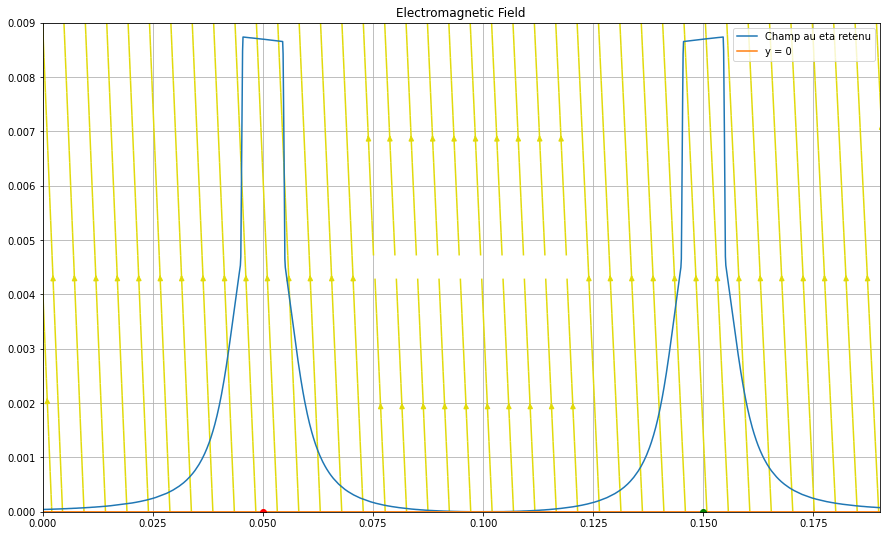
\includegraphics[width=.6\linewidth]{img_yamato/Hauteur.png}
        \captionof{figure}{Fonction $\eta$(x) obtenue grâce à la Méthode de Newton à partir de deux fils de courant inverse}
\end{figure}
\newpage
\textbf{\underline{Remarque :}} Ce même code exécuté en prenant comme champ magnétique la nappe de courant donne cette figure :

\begin{figure}[h]
	\centering
    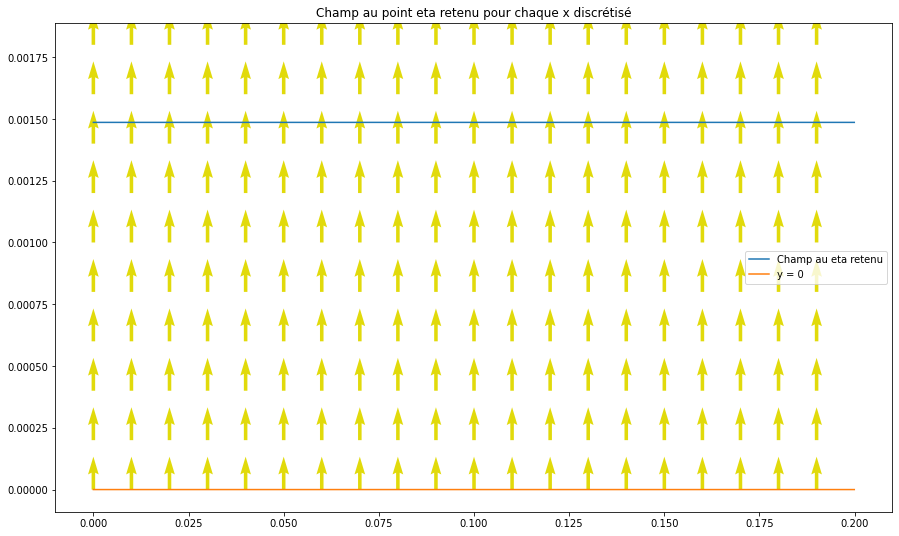
\includegraphics[width=.6\linewidth]{img_yamato/Nappe_plot.png}
        \captionof{figure}{Fonction $\eta$(x) obtenue grâce à la Méthode de Newton à partir de la nappe de courant}
\end{figure}
Le champ étant constant, il est normal de retrouver une fonction $\eta$(x) constante également.
\subsection{Résolution Générale}
Il s'agit maintenant de résoudre numériquement l'équation dans sa globalité. L'idée est de discrétiser en temps les termes $\eta$ et $\eta''$ en utilisant le \textbf{schéma des différences finies}. 
\begin{equation}
\eta'(t_n)=\frac{\eta(t_{n+1})-\eta(t_n)}{t_{n+1}-t_n} \indent
\eta''(t_n)=\frac{\eta(t_{n+1})-2\eta(t_n)+\eta(t_{n-1})}{t_{n+1}-t_{n-1}}
\label{eq29}
\end{equation}
Par la suite nous appliquons un schéma des différences finies explicite associé à un Newton (nous considèrons les autres termes de l'équation au temps $t_n$). Enfin, il s'agit de résoudre à chaque pas de temps l'équation à l'aide d'une méthode de Newton. Nous n'avons malheureusement pas eu le temps de l'implémenter.
\newline
Cependant, il n'y a pas de raison a priori pour que cela fonctionne... Nous pouvons essayer de faire cela en prenant un pas de temps assez petit, et de voir si la méthode converge en espace (en raffinant successivement le pas en espace). Puis regarder si la méthode converge en temps (en raffinant le pas en temps). Il peut aussi arriver que la méthode converge seulement si nous raffinons le pas d'espace et de temps en même temps, ou qu'il y ait une condition à respecter sur ces deux pas de discrétisation pour que la méthode converge (condition CFL par exemple). Pour être sûr du comportement de ce schéma aux différences finies, il faudrait faire son analyse numérique (regarder la consistante et la stabilité) en fonction des deux pas de discrétisation (chose que nous n'avons pas eu le temps de faire).
\newline
\newline
Une autre méthode peut aussi être envisageable en appliquant le schéma d'Euler explicité plus haut en y ajoutant le terme non linéaire. L'équation différentielle se réécrit alors de la manière suivante:
\begin{equation}
\frac{\gamma \eta\prime\prime}{(1+\eta^{2}\prime)^{\frac{3}{2}}} + (\rho_{1} - \rho_{2})g\eta +(\chi_1-\chi_2)*H^2=0
\end{equation}
Soit $\phi$ une application solution de \ref{eq29}. Alors $\phi$ est solution de \ref{eq29} si et seulement si :
\begin{equation}
t \mapsto\begin{pmatrix}
   \phi(x)  \\
   \phi\prime(x)
\end{pmatrix}=\begin{pmatrix}
	y_1 \\
	y_2
\end{pmatrix}
\end{equation}
est solution de (S)
\begin{equation}
(S) \Longleftrightarrow
\begin{cases}
y_1=y_2 \\
y_2=\frac{-(\rho_1-\rho_2)}{\gamma}gy_2-\frac{\chi_1-\chi_2}{\gamma}H^2
\end{cases}
\Longleftrightarrow
(y_1,y_2)=f(y_1,y_2)
\end{equation}
où f est la fonction suivante:
\begin{equation}
f: \begin{pmatrix}
y_1 \\
y_2
\end{pmatrix} \mapsto\begin{pmatrix}
	y_2 \\
	\frac{-(\rho_1-\rho_2)}{\gamma}gy_2-\frac{\chi_1-\chi_2}{\gamma}H^2
\end{pmatrix}
\end{equation}
D'où le schéma suivant:
\begin{equation}
\begin{cases}
u_{0} &=\begin{pmatrix}
   \eta(0)  \\
   \eta\prime(0)
\end{pmatrix} \\
u_{n+1} &= u_{n} + hf(u_{n})\\
\end{cases}
\Longleftrightarrow
\begin{cases}
u_{0} &=\begin{pmatrix}
   \eta(0)  \\
   \eta\prime(0)
\end{pmatrix} \\
\begin{pmatrix}
   \eta_{n+1}  \\
   \eta\prime_{n+1}
\end{pmatrix}  &= \begin{pmatrix}
   \eta_{n} +h \eta^{\prime}_{n}  \\
   \eta\prime_{n} - h \frac{(\rho_{1} - \rho_{2})g}{\gamma}\eta_{n}-\frac{(\chi_1-\chi_2)}{\gamma}H^2
\end{pmatrix}
\end{cases}
\end{equation}
Néanmoins il n'est pas certain que cela marche tel quel, il faudrait regarder en détail s'il ne faut pas des conditions plus restrictives que dans le schéma précédent sur le pas, les conditions initiales... pour assurer que ce que nous traçons est bien représentatif de la réalité physique.
\section{Bilan Ethique}
Notre projet s'inscrit dans un contexte d'application plus large, allant du milieu biomédical à l'écologie. En effet, ce type de fluide permettrait d'améliorer le quotidien de certains patients et de soigner d'une meilleur manière les maladies (extraction de molécule de cellules), comme présenté dans l'introduction. Également, les techniques de refroidissement ont connu, ces dernières années, un développement et un intérêt très important que ce soit au niveau de la recherche ou de l’industrie et les ferrofluides présentent aussi un intérêt dans ce domaine \cite{site3}.
\section{Bilan personnel}
\subsection{Mathieu Nguyen}
Ce projet a pu me permettre de mettre en place les différentes méthodes de résolution numérique vues en cours, mais cette fois-ci sur un problème physique. La partie la plus compliquée était de déterminer nous-même l'équation, contrairement en cours où la fonction est toujours donnée et/ou évidente. Une autre difficulté que j'ai rencontré est de programmer ces méthodes dans un autre language de programmation (C), et j'ai eu beaucoup de mal à voir comment appeler les différentes variables dans le code. Je devais à la base coder tout cela en C++, mais ne connaissant pas ce langage, je suis d'abord passé par le langage C, puis je l'ai retranscrit en C++, faisant donc outre des différents outils que le C++ offre par rapport au C, et c'est quelque chose que j'aurai beaucoup aimé approfondir.
\newline
Au final, j'ai pu comprendre que les méthodes numériques peuvent s'utiliser dans énormément de domaine, notamment dans tout le domaine physique où tout déplacement peut résulter en une équation différentiel non linéaire à résoudre numériquement. Cependant ce travail m'a forcé à me replonger dans le domaine de la magnétostatique, et ce n'est pas un domaine où je suis à l'aise. J'ai donc du compenser cela en effectuant beaucoup de recherches. Je reconnais cependant que je ne pensais pas qu'un champ magnétique serait capable de modifier la surface d'un fluide de la sorte, me permettant d'imaginer de nombreuses possibilités futures.
\subsection{Léo-Paul Baudet}
Ce projet m'a tout d'abord permis d'acquérir des connaissances supplémentaires en analyse numérique et d'envisager des méthodes d'analyse numérique plus sophistiquées, de part l'allure de l'équation qui sort du cadre classique vue en cours. De plus, le cadre d'application a aussi été enrichissant d'un point de vue intellectuel puisque celui--ci sort de nos matières de prédilection (électromagnétisme, statique des fluides, ...etc). Enfin, ce projet m'a aussi permis d'apprécier le travail en groupe particulièrement performant durant ce projet.
\subsection{Pauline Tournier}
Durant ce projet, nous avons pu aborder de nombreuses notions notamment toutes celles concernant les ferrofluides et l’électromagnétisme. Il nous a permis de mettre en parallèle et ainsi faire le lien entre des notions vues en cours et un sujet que nous ne connaissions pour la plupart très peu. Tout au long de ce projet, j’ai pu davantage cerner l’utilité de certaines méthodes dans la résolution de problèmes numériques et encore une fois approfondir mes connaissances informatiques, ici en Python. Notre groupe a pu progresser ensemble et s’entraider afin d’arriver aux résultats espérés, ce qui a permis de renforcer notre aptitude au travail d’équipe. En conclusion, bien que très technique, ce projet s’est avêré être très enrichissant, et m’a permis de revoir et d’acquérir de nouvelles notions.
\subsection{Lucie Miniaou}
Lors de ce projet j’ai pu travailler en binôme avec Pauline sur la partie résolution d’équation différentielle linéaire. Cela m’a permis d’appliquer les méthodes vues au cours de l’année sur un projet concret notamment la méthode d’Euler explicite vue au premier semestre. De plus, notre encadrant a su nous guider et nous a appris à toujours remettre en question et se questionner sur les résultats obtenus. C’est pourquoi ce travail a été très enrichissant malgré la difficulté du sujet.

\section{Conclusion}
Pour conclure, dans ce projet nous n'avons résolu qu'une partie du projet initial: nous avons mis au point une résolution numérique dans deux cas particuliers afin d'une part de valider nos schémas numériques par rapport à la réalité physique et d'autre part d'envisager sur des cas plus simple des stratégies de résolutions. Il reste maintenant à recoller ces schémas en introduisant dans le schéma d'Euler validé plus haut la partie non linéaire de l'équation ou bien à déterminer une stratégie de résolution plus générale (différences finies par exemples). Néanmoins, il n'est pas certain à priori que le recollement fonctionne directement, il faudrait peut être vérifier des conditions supplémentaires au niveau du pas, des conditions initiales, des paramètres du système physique pour que celui-ci reste valable.


\part*{Annexe}
\addcontentsline{toc}{part}{Annexe :}

Tous nos codes  et références sont regroupés sur GitHUB au lien : \href{https://github.com/Yamacia/Ferrofluide/tree/master}{Lien GitHUB}
\newline
Le dossier \textbf{equation\_sans\_champs} correspond à la section (6.1), les codes sont en Python et permettent de résoudre toutes les équations considérées pour résoudre l'équation sans champ magnétique, ainsi que pour les afficher.
\newline
Le dossier \textbf{equation\_sans\_differentiel} correspond lui à la section (6.2), où les codes sont également en Python. La conversion en C et C++ de ces fichiers sont eux dans le dossier \textbf{Code}. Ces codes regroupent 2 méthodes différentes de résolution numérique, la \textbf{méthode de dichotomie} et la \textbf{méthode de Newton}, mais nous avons principalement utilisé la méthode de Newton, car elle permettait une meilleure précision.
\newline
Le fichier \textit{code.c} regroupe tous les fonctions que nous avons créé pour résoudre notre équation et exporter nos valeurs dans ces fichiers textes.\\
Le fichier \textit{code.h} est notre header et regroupe toutes les fonctions crées, toutes les bibliothèques utilisées ainsi que les \textbf{constantes que nous avons défini}. \\
Le fichier \textit{main.c} est lui le programme main nous permettant d'exécuter tous les codes. \\
Nous avons également un \textit{Makefile succinct} pour plus facilement compiler tous ces fichiers. \\
Le fichier \textit{graphes.ipynb} est lui un fichier Python nous permettant de créer nos graphiques.
\newline
Tous les fichiers créés pour programmer en C ont également été dupliqué en version C++ car, pour une raison étrange, notre éditeur de texte ne voulait pas fonctionner lorsque nous codions en C, mais marchait correctement en C++. Le nom de chaque fichier reste le même, seule l'extension change.
\newline
Les différents documents qui nous ont servi en tant que documentation sont regroupés dans le dossier \textbf{Cours}, et sont essentiellement des documents que notre professeur nous a envoyé. Les autres documents utilisées sont explicités dans les \textbf{références}.
\newpage
%-----------------------------------------------------------
\bibliography{bibliographie.bib}
\bibliographystyle{unsrt}

\end{document}